\documentclass[twocolumn]{scrartcl}

\include{header/zusammenfassung}
\usepackage{tikz}
\usepackage{adjustbox}
\usetikzlibrary{arrows}
\usetikzlibrary{calc}

\DeclareMathOperator{\Ref}{\text{ref}}
\DeclareMathOperator{\In}{\text{in}}
\DeclareMathOperator{\Out}{\text{out}}


\title{MikroelSys2 Zusammenfassung}
\subtitle{Dozent: G.Keel}
\author{H.Badertscher}

\begin{document}
\selectlanguage{ngerman}

\onecolumn

\maketitle

\newpage

\tableofcontents

\twocolumn


\section{Messung von Kapazitäten}

\subsection{Stromquelle}
Prinzip: Kapazität wird mit einem Strom $I_0$ während einer fixen Zeit 
$t_0$ aufgeladen. Die Kapazität berechnet sich aus
\begin{equation*}
	V_{\Out} = C_x \cdot I_0 \cdot t_0
\end{equation*}
Diese Art der Messung benötigt eine präzise Stromquelle oder eine
Referenzkapazität. Weiter werden sehr kleine Ströme benötigt, was
diese Methode für PCB-Design unpraktikabel macht. Im IC-Design
ist eine Messung mit Stromquellen gut möglich.

\subsection{RC-Oszillator}
Mit einem Timer-Baustein, wie z.B. LM555 wird ein Oszillator aufgebaut,
dessen Oszillatorfrequenz gemessen wird. Für den LM555 beträgt die Frequenz

\begin{equation*}
	f = \frac{1}{0.693 \cdot C_1 \cdot (R_1 + 2 R_2) }
\end{equation*}

\subsection{AC-Widerstand / Phasenverschiebung}
Die Phasenverschiebung wird gemessen, indem mit einer Sinusquelle das RC-Netzwerk,
bestehend aus der Messkapazität $C_x$ und einem bekannten Widerstand $R$,
angeregt wird und die Phasenverschiebung mittels eines Lock-In Verstärkers
gemessen wird.

\begin{multicols}{2}
	\centering
	\begin{circuitikz}[scale=0.6,transform shape]

	\draw	(0,-2) to[sV] (0,0)
			(0,0) to[R,l={$R$}] (2,0)
			(2,0) to[C,l={$C$}] (2,-2)
			(0,-2) to (2,-2)						
			(2,0) to (3,0) node[ocirc] {}
			(2,-2) to (3,-2) node[ocirc] {};

\end{circuitikz}
	
	\vfill\columnbreak
	\begin{align*}
		H(s) &= \frac{1}{1+sRC} \\
		\left|H(\omega)\right| &= \frac{1}{\sqrt{1+\left(\omega RC\right)^2}} \\
		\Theta(\omega) &= -\arctan\left(\omega RC\right)
	\end{align*}
\end{multicols}

\begin{align*}
	& \text{Eingangssignal} & f_{\In}(\varphi,t) &= \sin(\omega_0 t + \varphi) \\
	& \text{Sync-Signal} & f_{\text{sync}}(t) &= \sin(\omega_0 t) \\
	& \text{Produkt} & f_{\text{mod}}(\varphi,t) &= \sin(\omega_0 t + \varphi) \cdot \sin(\omega_0 t) \\
	& & &= \frac{\cos(\varphi)}{2} - \frac{\cos(\varphi + 2 t \omega_0)}{2}
\end{align*}

Der Mittelwert von $f_{\text{mod}}$ über eine Periode beträgt also
\begin{equation*}
	\bar{f}_{\text{mod}} = \frac{\cos(\varphi)}{2}
\end{equation*}
womit sich die Phase des Eingangssignals $f_{\In}$ bestimmen lässt. \\

Das gleiche Verfahren funktioniert auch mit einem Synchrongleichrichter. 
Dabei wird das Eingangssignal mit einem zum Sinus phasengleichen Rechtecksignal
multipliziert:
\begin{align*}
	f_{\text{mod}}(\varphi,t)) &= \text{sgn}\left(\sin(\omega_0 t)\right) \cdot \sin(\omega_0 t + \varphi) \\
	V_{\text{int}} &= A \frac{2 \sin \varphi}{\pi} \frac{T_{\text{int}}}{R C}
\end{align*}
Damit ergibt sich über eine Periode integriert
\begin{equation*}
	\bar{f}_{\text{mod}} = \frac{2 \cos(\varphi)}{\pi}
\end{equation*}

Damit werden Frequenzen geradzahliger Vielfacher ($2,4,...$) vom Integrator
ausgelöscht, während ungeradzahlige Vielfache um den Faktor $1/n$
abgeschwächt werden.

\subsection{Ladungsverstärker}
Eine Kapazität $C_x$ wird mit einer bekannten Spannung geladen. Die resultierende
Ladung beträgt
\begin{equation*}
	Q_x = C_x \cdot V_{\Ref}
\end{equation*}
Die Kapazität wird nun auf eine bekannte Kapazität $C_{\Ref}$ entladen. 
Es resultiert die Ausgangsspannung
\begin{equation*}
	V_{\Out} = - \frac{Q_x}{C_{\Ref}} = \frac{C_x}{C_{\Ref} V_{\Ref}}
\end{equation*}

\newpage
\section{Aktive Filter}

\subsection{Filter 1. Ordnung}

\subsubsection{Integrator}
\begin{multicols}{2}
	\begin{center}
		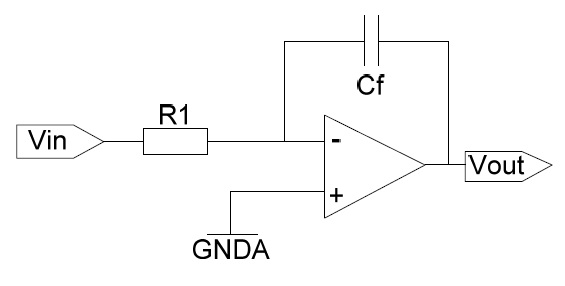
\includegraphics[width=6cm]{images/filter_1_integrator.jpg}
	\end{center}
	\begin{align*}
		T(s) &= Y_{\In} \Zop = - \frac{1}{s C_f R_1} \\
		V_{\Out} &= -\frac{1}{R_1 C_f} \int V_{\In} dt + V_0
	\end{align*}
\end{multicols}

\subsubsection{Tiefpass}
\begin{multicols}{2}
	\begin{center}
		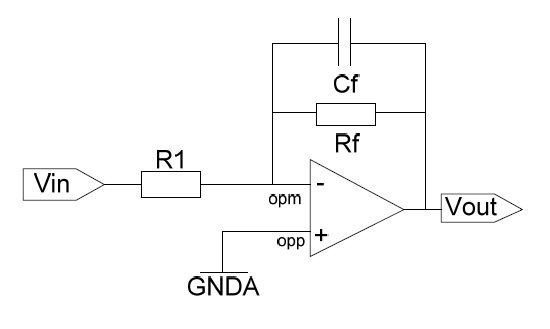
\includegraphics[width=6cm]{images/filter_1_tiefpass.jpg}
	\end{center}
	\begin{align*}
		T(s) &= -\frac{R_f}{R_1} \cdot \frac{1}{1 + s C_f R_f}
	\end{align*}
\end{multicols}

\newpage
\subsubsection{Differenzierer}
\begin{multicols}{2}


	Achtung: dieser Differenzierer schwingt meistens.
	\begin{center}
		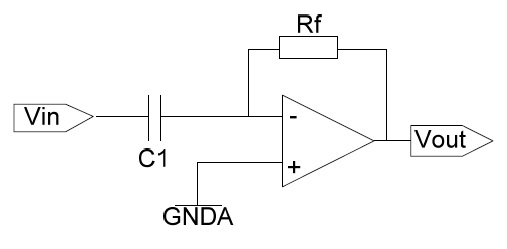
\includegraphics[width=6cm]{images/filter_1_diff.jpg}
	\end{center}
	\begin{align*}
		T(s) = -s C_1 R_f
	\end{align*}
\vfill	
\columnbreak
	Bandpass mit differenzierendem Frequenzbereich
	\begin{center}
		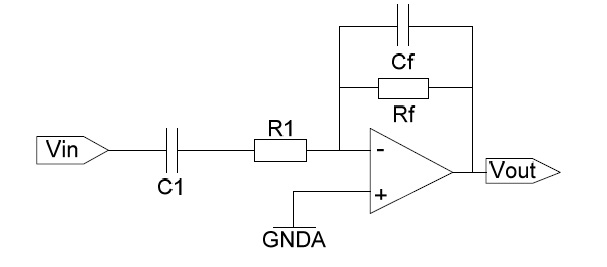
\includegraphics[width=0.7\linewidth]{images/filter_1_diff2.jpg}
	\end{center}
	\begin{align*}
		T(s) = - \frac{s C_1 R_f}{1 + s C_1 R_1} \cdot \frac{1}{1 + s C_f R_f}
	\end{align*}
	Differenziert zwischen $\omega_1 = \frac{1}{R_1 C_1}$ und 
	$\omega_2 = \frac{1}{R_f C_f}$

\end{multicols}

\subsection{Filter höherer Ordnung}

\begin{multicols}{2}
	\paragraph{Tiefpass 2. Ordnung}
	\begin{equation*}
		T_{TP}(s) = \frac{A \omega_0^2}{s^2 + \frac{\omega_0}{Q} s + \omega_0^2}
	\end{equation*}
	
	\paragraph{Bandpass 2. Ordnung}
	\begin{equation*}
		T_{BP}(s) = \frac{A \frac{\omega_0}{Q} s}{s^2 + \frac{\omega_0}{Q} s + \omega_0^2}
	\end{equation*}
\end{multicols}


\subsubsection{Sallen-Key Filter}
\paragraph{Sallen-Key Tiefpass}
\begin{center}
	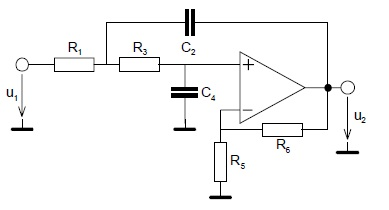
\includegraphics[width=8cm]{images/filter_sk_tp.jpg}
\end{center}
\begin{equation*}
	T(s) = \frac{A}{1 + \left(R_3 C_4 + R_1 C_4 + R_1 C_2 (1-A)\right) \cdot s + R_1 R_3 C_2 C_4 \cdot s^2}
\end{equation*}

\paragraph{Sallen-Key Bandpass}
\begin{center}
	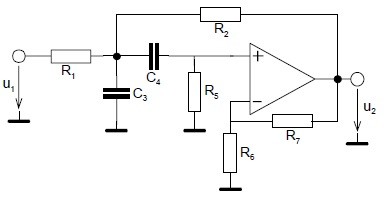
\includegraphics[width=8cm]{images/filter_sk_bp.jpg}
\end{center}
\begin{equation*}
	T(s) = \frac{\frac{R_2 R_5}{R_1 + R_2} C_4 A_M \cdot s}{1 + \frac{R_1 R_5 C_4 (1-A_M) + R_1 R_2 (C_3 + C_4) + R_2 R_5 C_4}{R_1 + R_2} \cdot s + \frac{R_1 R_2}{R_1 + R_2} R_5 C_3 C_4 \cdot s^2}
\end{equation*}
mit $A_M = 1+\frac{R_7}{R_6}$

\subsubsection{Multiple Feedback Filter}
\begin{center}
	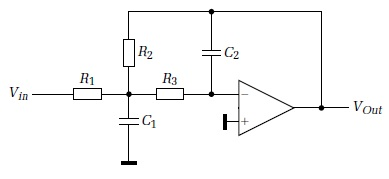
\includegraphics[width=8cm]{images/filter_mfb.jpg}
\end{center}
\begin{align*}
	T(s) &= \frac{G_0}{1 + C_s \left(R_2 + R_3 + R_3 \frac{R_2}{R_1}\right) \cdot s + C_1 C_2 R_2 R_3 \cdot s^2} \qquad \text{mit} \quad G_0 = -\frac{R_2}{R_1} \\
	Q &= \frac{\sqrt{C_1 C_2 R_2 R_3}}{C_2 \left(R_2 R_3 R_3 \frac{R_2}{R_1}\right)}
\end{align*}
Die Güte wird v.a. mit $C_2$ und $R_1$ eingestellt.


\subsection{Biquads}
Beispiel Bandpass:
\begin{center}
	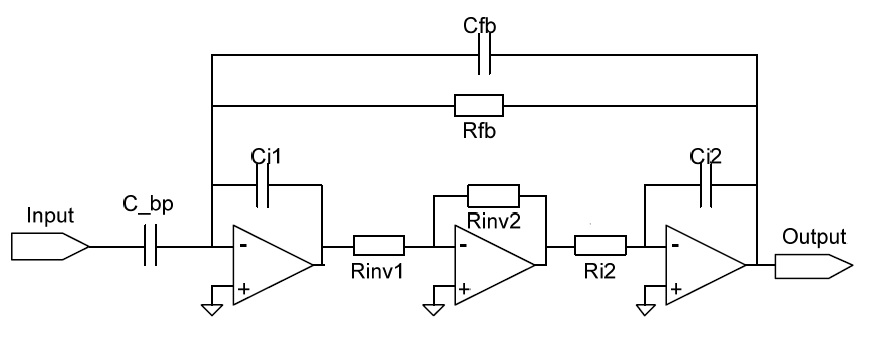
\includegraphics[width=8cm]{images/filter_biquad.jpg} 
	\hspace{2cm}
	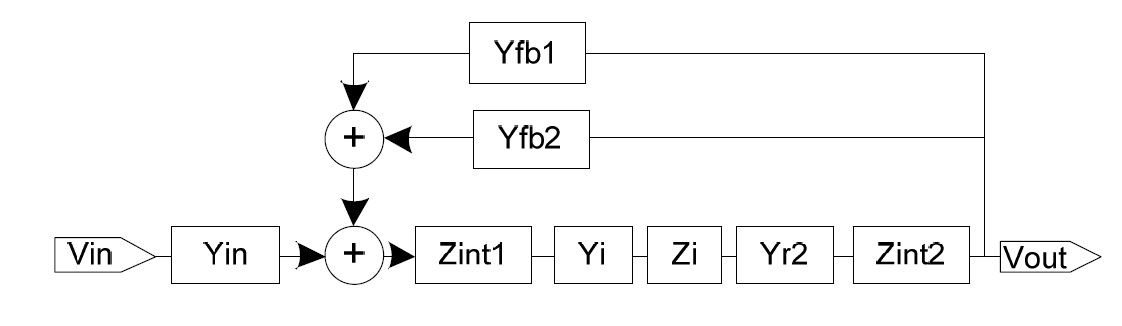
\includegraphics[width=8cm]{images/filter_biquad_block.jpg} 
\end{center}
\begin{align*}
	T(s) &= \frac{Y_{\In} Z_{\Int 1} Y_i Z_i Y_{r 2} Z_{\Int 2}}{1 - (Y_{\Fb 1}+Y_{\Fb 2}) Z_{\Int 1} Y_i Z_i Y_{r 2} Z_{\Int 2}}
	&= \frac{\frac{C_{bp}}{C_{i1} R_{i2} C_{i2}} \cdot s}{s^2 + \frac{C_{fb}}{C_{i1} R_{i2} C_{i2}} \cdot s + \frac{1}{R_{fb} C_{i1} R_{i2} C_{i2}}}
\end{align*}
und damit
\begin{equation*}
	A = -\frac{C_{bp}}{C_{fb}} \qquad Q = \sqrt{\frac{R_{i2}}{R_{fb}}} \cdot \frac{\sqrt{C_{i1} C_{i2}}}{C_{fb}} \qquad f_0 = \frac{1}{2 \pi \sqrt{C_{i1} C_{i2} R_{fb} R_{i2}}}
\end{equation*}

%TODO: Tiefpass, Abgeänderte Version, Tow Thomas, Ackerberg-Mossberg

\newpage
\section{Switched Capacitor Schaltungstechnik}

\newpage
\section{Spezielle Operationsverstärker}

\newpage
\section{Sigma-Delta Wandler}

\subsection{Pattern Noise}
DC-Eingangsspannungen führen zu repetitiven Sequenzen am Modulator-Ausgang, so genanntem Pattern Noise.
Ist $x$ sehr klein, entstehen repetitive Sequenzen tiefer Frequenz.
\begin{center}
	\begin{tabular}{ll}
		\textbf{Eingangsspannung} & \textbf{Pattern Noise Periode} \\ \hline
		$V_{\In} = 0$ & $\frac{1}{2} \Fclk$\\
		$V_{\In} = \pm \frac{1}{2} V_{\Ref}$ & $\frac{1}{4} \Fclk$ \\
		$V_{\In} = \pm \frac{1}{8} V_{\Ref}$ & $\frac{1}{16} \Fclk$ \\
		$V_{\In} = \pm 0.1 V_{\Ref}$ & $\frac{1}{20} \Fclk$ \\
		$V_{\In} = x \cdot V_{\Ref}$ & $\frac{x}{2} \Fclk$\\
		\hline
	\end{tabular}
\end{center}


\subsection{Signal-Rausch-Abstand}

Für einen $n$-bit Modulator bei einer Signalfrequenz von $f_0$ kann das Rauschen wie folgt berechnet werden:
\begin{flalign*}
	&\text{Signal-to-Noise Ratio} && \text{SNR} && \approx -3.4 + 6 n + 9 \log_2\left(OSR\right) \\
	&\text{Oversampling Ratio} && \text{OSR} && = \frac{f_s / 2}{f_0} \\
	&\text{Effektivwert $n_0$ der Rausch-Spannung für Ordnung $n=1$} && n_0 && \approx \frac{q}{\sqrt{12}} \frac{\pi}{\sqrt{3}} \left(\frac{2 f_0}{f_s}\right)^{3/2} \\
	&\text{Effektivwert $n_0$ der Rausch-Spannung für Ordnung $n=2$} && n_0 && \approx \frac{q}{\sqrt{12}} \frac{\pi^2}{\sqrt{5}} \left(\frac{2 f_0}{f_s}\right)^{5/2} \\
	&\text{Effektivwert $n_0$ der Rausch-Spannung für Ordnung $n=3$} && n_0 && \approx \frac{q}{\sqrt{12}} \frac{\pi^3}{\sqrt{7}} \left(\frac{2 f_0}{f_s}\right)^{7/2} \\
\end{flalign*}

\newpage
\section{Sensorsysteme}



\end{document}
